\section{Introduction}
In parallel to the investigations of vicinal (100) substrates, the ARISE project investigated alternative substrate orientations including (111) and (211). While the results of (111) substrates were uninteresting, growth of thin films on (211) substrates demonstrated a number of interesting properties. Most interesting amongst these was the spontaneous tilting of thin films grown on top of (211) oriented silicon substrates. Such tilting had been remarked upon previously in literature,  but no comprehensive examination of its origins or relationship to material parameters had been examined.

In this work, also done in close collaboration with Ms. Steffi Woo, the spontaneous tilting of thin films grown on (211) oriented silicon substrates was examined. The effects of the naturally asymmetric substrate was found to cause a tilt of the growing thin film in order to minimize the strain across the interface. Using this idea of projected strain minimization across the interface, a model was developed which predicted the tilt as a function of intrinsic lattice mismatch between the substrate and thin film. Examiniation of the reports of thin film tilting in literature showed the model successfully calculated tilt for a large number of material systems and made predictions for those systems for which no measured values had been reported.
\section{Background}
The (211) orientation of non-polar semiconductor substrates, most notably silicon, has a number of beneficial properties. Of most relevance to the epitaxy of thin films on Si(211) substrates is the occurrence of two energetically non-equivalent lattice sites on the surface, without the need for surface reconstruction.\cite{Wright1982} These two non-equivalent lattice sites offer preferential nucleation locations for the individual adatoms during growth of polar (group III-V and II-VI) semiconductors. Such preferred nucleation is proposed to eliminate the occurrence of anti-phase domains (APDs) during the growth of polar semiconductors\cite{Wright1982} while also maintaining the interface neutrality condition of h$\pm$k$\pm$l$=$0.\cite{Wright1982} The intrinsic asymmetry of the (211) surface is also expected to influence the formation of epitaxial twins during growth\cite{Devenyi2011}. Si(211) substrates have been used to produce the highest quality CdTe\cite{Zhao2011}, ZnTe\cite{Wang2011a} and HgCdTe\cite{Dhar1997a} despite large lattice mismatches of 19.4\%, 12.3\%, and 19.1\%, respectively. 

Thin films grown on (211) substrates have been previously observed in literature to have a tilted epilayer orientation relative to the substrate.\cite{Zhao2011,Wang2006,Dhar1997a,Lange1991,Nakamura1992} The tilt phenomenon has been attributed to a number of causes by different authors including the glide and interactions of misfit dislocations \cite{Olsen1975,Riesz1994,Ayers1991,Johnson2011} and localized distortion of the lattice at the interface.\cite{Sasaki1992} The mechanisms proposed thus far have been unsuccessful at predicting the tilt of mismatched epilayers over large range of mismatch (0--20\%) found in III-V and II-VI material systems. A phenomenon intimately intertwined with tilted epitaxy is ``dual epitaxy'', observed by numerous authors\cite{Li1995a,Nakamura1992,Rujirawat1998,Lange1991} that mismatched CdTe on GaAs(211) epitaxy can result in films growing in a twinned orientation, combined with a tilt; such that the (133) planes make up the epilayer surface and are parallel to the substrate (211) planes. The tilt component of dual epitaxy is same tilt phenomenon examined here.

\section{Experimental}
GaSb thin films were deposited on nominal (211)-oriented Si substrates, according to our previously published procedures\cite{Devenyi2011}, at 600, 640 and 500\degreeC. Two dimensional X-ray diffraction (2DXRD) frames were captured for stereographic pole figure analysis and crystallographic indexing as per Devenyi \textit{et al.}\cite{Devenyi2011}.
\begin{figure}
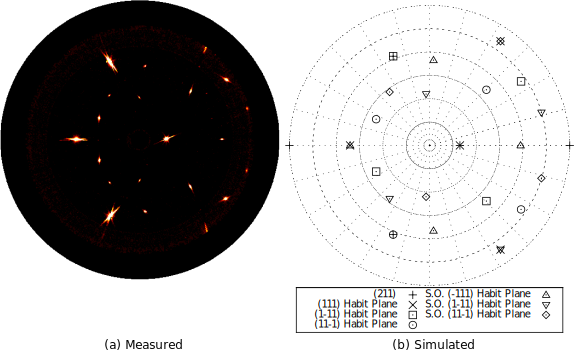
\includegraphics{211_polefigure}
\caption{\label{fig:211_polefigure}a) 2DXRD Stereographic pole figure and b) accompanying modelled pole figure, identifying the origin of each peak in the pole figure from the bulk or one of six twin variants. Overlapping peaks indicate twinning habit planes. Outermost poles are partially visible due to experimental limitations. Streaking in peaks is due to instrumental broadening. (S.O. = second-order twinning).}
\end{figure}
\section{Results}
2DXRD data was processed into a GaSb (111) pole figures as shown in FIG.~\ref{fig:211_polefigure}, representing a stereographic projection of all $<$111$>$ spacings present in the GaSb epilayer. Modeling (as per Devenyi \textit{et al.}\cite{Devenyi2011})\ of the poles present indicate that there are seven phases of GaSb, the bulk (211) orientation of GaSb and six twin variants, three first-order twins and three second-order twins from the twin variant with (111) habit plane, with 58\%, 21\% and 2\% of the intensity (and hence volume fraction) present in the twinned orientation for the films presented here. Volume fractions were determined by integration of the sum of intensity of unique (111) X-ray peaks from all twinned orientations, and divided by total intensity of all unique (111) reflections (sum of bulk and twin intensities), performed using \textit{Bruker GADDS}. There are two distinct nomenclatures used in literature to describe phases present in epitaxial films.\cite{Kim2010a,Lange1991,Johnson2011,DeLyon1995} One method describes the crystallographic direction which is normal to the surface for each phase, while the other (which the authors choose to employ here) describes the nature of the crystallographic orientation relationship between the secondary phases with respect to the orientation of the substrate. Where reference is made to literature using the first, descriptions will be translated into the second for ease of comparison.

Indexing of the crystal unit cells present in the film was performed using \textit{Bruker APEXII} single crystal refinement software, to obtain orientation matrices for the Si substrate as well as the seven GaSb phases. The bulk thin film orientation matrix was then compared to the substrate matrix and a tilt calculated using \textit{orilib} a crystal orientation calculation library, yielding a tilt of 2.65\degree, 2.55\degree and 2.40\degree $\pm$ 0.2\degree about the [01$\overline{1}$] direction towards [$\overline{1}$11], these values are indistinguishable within experimental error. The (111) habit plane twin formed in these films is also tilted with respect to the substrate, by the same angle as the bulk, this is expected by crystallography, since this twinned orientation shares extended interfaces with the bulk orientation.
\begin{figure}
\includegraphics{211_tem}
\caption{\label{fig:211_tem}Conventional TEM image of the (0$\overline{1}$1) cross section, with inset diffraction pattern of the epitaxial and (111) habit plane twin variant in blue and red, respectively, and inset higher-magnification of the epitaxial variant showing misfit dislocations.}
\end{figure}

Two transmission electron microscopy (TEM) cross-sections were prepared, in orthogonal directions of [0$\overline{1}$1] and [1$\overline{1}\overline{1}$]. The specimens were prepared by conventional mechanical polishing and ion milling, and examined as described in Woo \textit{et al.}\cite{Woo2012} Conventional TEM imaging of the (0$\overline{1}$1) cross-section of the epilayers, combined with the selected area electron diffraction (SAED) pattern of the [0$\overline{1}$1] zone axis as shown in FIG.~\ref{fig:211_tem} confirms the presence of microtwins with (111) habit planes. These microtwins are observed in the perpendicular (1$\overline{1}\overline{1}$) cross-section as large bands lying parallel to the interface over a long-range, alternating with the epitaxial variant (not shown). The observed misorientation between the GaSb and Si reflections in the [0$\overline{1}$1] SAED pattern also indicate a tilted epilayer (both epitaxial and twin variants) with a tilt of 2.54$^\circ \pm 0.2^\circ$ towards the [$\overline{1}$11] direction. The 133 reflection of the twinned GaSb nearly coincides with the Si substrate normal 422 reflection. The GaSb twin variant can be differentiated in real space by selective dark-field imaging formed using one of the twinned reflection spots. The jagged features at the GaSb/Si interface (seen in detail in the inset of FIG.~\ref{fig:211_tem}) only belong to the epitaxial variant. This is indicative of the presence of misfit dislocations at the portions of the interface where the epitaxial region meets the substrate, as characterized by Vajargah \textit{et al.}\cite{Vajargah2011b}
\section{Discussion}
Analysis using an atomic ball-and-stick model, along with trigonometric modelling of lattice plane spacing, can be used to demonstrate that the tilted epitaxy reduces the projected in-plane lattice strain along one dimension for the GaSb/Si system. FIG.~\ref{fig:211_model} shows the alignment of planes present in the epitaxial and twinned variants of the GaSb epilayer. The Si(111) plane spacing (in red) at an angle of 19.471\degree to the Si(211) surface is aligned to the GaSb(111) plane spacing (in blue), by a tilt of 2.50\degree in the epilayer. The relationship describing zero projected strain condition between these planes across the interface is described in EQN.~\ref{eqn:211_epi} for the case of $a_{Sub} = a_{Si}$ and $a_{Film} = a_{GaSb}$, where $\delta$ is the tilt angle. This relationship (dot-dash line) also applies over the full range of common heteroepitaxial lattice mismatches grown on (211) substrates, from GaP/Si to CdTe/Si, as shown in FIG.~\ref{fig:211_data}.
\begin{gather} 
 \frac{ a_{film}}{\sqrt{3} \sin(19.471^\circ + \delta)} = \frac{a_{Sub}}{\sqrt{3}\sin(19.471^\circ)} \label{eqn:211_epi}\\
 \frac{ a_{film}}{2\sin(74.207^\circ + \delta)} = \frac{ a_{Sub}}{\sqrt{3}}   \label{eqn:211_twin}
\end{gather}
\begin{figure}
\includegraphics{211_model}
\caption{\label{fig:211_model}Ball-and-stick atomic model of a triple junction of the epitaxial orientation, twinned orientation (with (111) habit plane in blue), and the Si(211) surface. Geometrical alignment of the atomic planes as described by EQNs.~\ref{eqn:211_epi} and \ref{eqn:211_twin} are also shown in red/blue and black, respectively. Terrace (T) and edge (E) atom labels denote the two non-equivalent surface sites.}	
\end{figure}
\begin{figure}
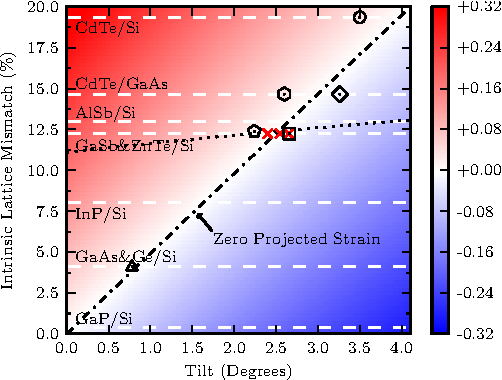
\includegraphics{211_data}
\caption{\label{fig:211_data}Colormap showing the projected strain as a function of intrinsic lattice mismatch and positive tilt angle of an epitaxial film, computed from EQN.~\ref{eqn:211_epi} with the zero projected strain contour highlighted (dot-dash line). The dotted line also overlays EQN.~\ref{eqn:211_twin}. Experimental data points from this work ($\times$), Ref.~\onlinecite{Zhao2011} ($\odot$), Ref.~\onlinecite{Wang2011a} ($\boxdot$), Ref.~\onlinecite{Johnson2011} ($\Diamond$, $\bigtriangleup$) and Ref.~\onlinecite{smith2012_znte,smith2012_gaas} ($\pentagon$, $\varhexagon$) are shown, indicating good agreement with measured tilts of thin films. Common heteroepitaxial systems are also highlighted. Close lattice mismatches are merged for figure clarity.}
\end{figure}
In the twinned orientation, the Si($\overline{1}$11) plane spacing is aligned to the projection of the GaSb(200)$_{tw}$ plane spacing (both in black) onto the GaSb/Si interface, by a tilt of 2.22\degree. The geometrical constraints of these planes can be described by the relations as expressed in EQN.~\ref{eqn:211_twin}. The line of zero projected strain for the twinned region is also shown in FIG.~\ref{fig:211_data} (dotted line). The applicability of EQN.~\ref{eqn:211_twin} is considerably more limited across heteroepitaxial systems, as the constraints described by EQN.~\ref{eqn:211_epi} also needs to be simultaneously satisfied as extended interfaces are shared. However, an equivalent relationship describing another set of planes for other lattice mismatches may replace the relationship described by EQN.~\ref{eqn:211_twin}. The proposed ball-and-stick atomic model (FIG.~\ref{fig:211_model}) also shows that the Ga- and Sb-atoms in the twinned variant are perfectly registered with the terrace (T) and edge (E) atoms of the Si substrate. The epitaxial variant interface is significantly distorted, and the same atomic registration of Ga- and Sb-atoms to the underlying Si substrate does not occur, however the projected sublattice is still aligned. This correlates well with the misfit dislocations observed at the GaSb/Si interface in the inset of FIG.~\ref{fig:211_tem}.

For general case of an epilayer with unknown twin volume-fraction, the tilt is bounded by competing factors of minimizing strain in both the epitaxial and twinned variants (as in GaSb on Si), with the projected strain effectively minimized at the volume-fraction weighted average of the two tilts. For GaSb with 58\%, 21\% and 2\% twin fraction, the predicted tilts are 2.493\degree, 2.498\degree and 2.500\degree. This small variation in tilt angle is due to the steeper slope of EQN.~\ref{eqn:211_epi}, thus its contribution dominates the weighted average. The intrinsic +12.2\% lattice mismatch between GaSb and Si is minimized, however there are localized strain variations between the epitaxial and twinned regions. For a film with 58\% twin, the projected (111) d-spacing in the epitaxial region is +0.03\% (in compression), while the projected GaSb(200) and Si($\overline{1}$11) d-spacing in the twinned region is -0.12\% (in tension). Thus, the proposed driving force for the tilted epilayer during growth is the minimization of lateral strain of close-packed (111) planes (red/blue planes in FIG.~\ref{fig:211_model}), in one dimension within the two-dimensional projected interface net.

In addition to accounting for the tilt observed for GaSb on Si, this model predicts the tilts observed in several other material systems. The growth of CdTe on Si(211) and GaAs(211) is a common use to buffer the growth of HgCdTe for detector applications. Several authors\cite{Triboulet2009,Yu1999,Lange1991} published results which indicate CdTe epilayers which are tilted in the range of 3.5\degree on Si(211)\cite{Zhao2011} and 3.26\degree on GaAs(211)\cite{Johnson2011}, about the [01$\overline{1}$] direction towards [$\overline{1}$11]. The direction and magnitude reported by those authors agrees well with the tilt of 3.97\degree and 3.00\degree, respectively, as predicted by this model. Discrepancy between the predicted and reported value of tilt is expected to be partially due to the presence of twinning in the epilayer, along with uncertainty in the reported values.

ZnTe is often used as an intermediate buffer epilayer, prior to the growth of CdTe and HgCdTe on Si(211).\cite{Zhao2011,Dhar1997a} Wang \textit{et al.}\cite{Wang2011a} published results which indicate epilayer tilts in the range of 2.66\degree while Smith \textit{et al.}\cite{smith2012_znte} reports tilts of 2.24\degree. This is in good agreement to the predicted value of 2.50\degree obtained from the proposed model. The good matching between our predicted and the reported values of tilt in ZnTe on Si(211) is expected to be due to the substantially low degree of twinning observed.

The model also makes a prediction of the tilt expected from the growth of GaAs on Si(211), a value of 0.83\degree is predicted. A tilt of 0.781\degree is reported by Johnson \textit{et al.}\cite{Johnson2011} when grown alone, and 0.835\degree when capped subsequently with CdTe, again demonstrating good agreement with the model.

For the systems AlSb/Si, InP/Si and GaP/Si, the model predicts tilt angles of 2.65\degree, 1.64\degree and 0.07\degree. Measurements of these material systems are expected to yield tilts that quantitatively follow this model.
\section{Implications for Symmetry and Energy at Epitaxial Surfaces}
